\subsection{Installation der Virtuellen Maschinen}
Die drei virtuellen Maschinen werden unter Oracle VirtualBox entsprechend Tabelle \ref{tab:host-config} installiert. Die Installationen erfolgen mit den jeweiligen grafischen Installern, wobei grundsätzlich die Standardeinstellungen verwendet werden. Für die beiden Debian-Systeme wure keine Desktopoberfläche ausgewählt (lediglich \inlinecodee{standard system utilities}). Abb. \ref{fig:vbox-group} zeigt die virtuellen Maschinen unter Virtualbox.

\begin{figure}[h]
  \centering
  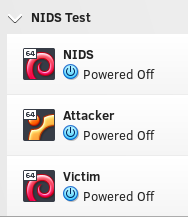
\includegraphics[width=0.2\textwidth]{graphics/setup/vbox_group.png}
  \caption{Verwendete Maschinen in Virtualbox.}\label{fig:vbox-group}
\end{figure}

\subsection{Snort-Installation}

Als nächstes wird snort auf der NIDS-VM installiert.
\begin{minted}{bash}
  su
  apt install snort
\end{minted}

Bei der Installation erscheint ein Konfigurationsfenster. In dieses muss die CIDR-Adresse des VirtualBox-Netzwerkes (\inlinecodee{192.168.56.0/24}) eingetragen werden (Abb. \ref{fig:snort-first-time-setup}).

\begin{figure}[H]
  \centering
  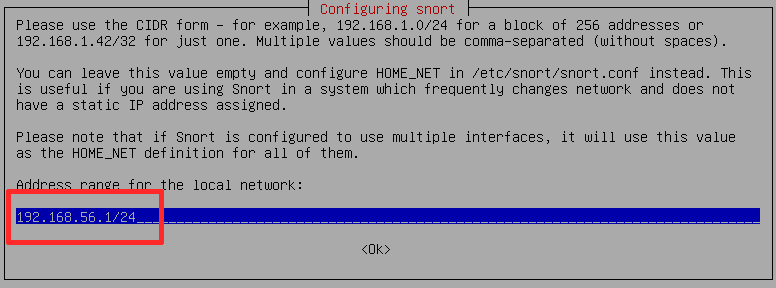
\includegraphics[width=0.5\textwidth]{graphics/setup/config-snort-1.png}
  \caption{Snort Konfiguration bei der Installation.}\label{fig:snort-first-time-setup}
\end{figure}

Mit dem folgenden Befehl kann die snort-Installation überprüft werden.
\begin{minted}{bash}
  /sbin/snort --version
\end{minted}

\subsection{Webserver-Installation}
\inlinecodee{nginx} wird auf dem Victim-Host als Ziel für den Angreifer installiert. Dazu wird lediglich folgender Befehl ausgeführt.
\begin{minted}{bash}
  su
  apt install nginx
\end{minted}

\subsection{Erstellen des Virtuellen Netzwerkes}
Um das virtuelle Netzwerk einzurichten, öffnet man zunächst \inlinecodee{File -> Tools -> Network Manager} und erstellt ein neues Netzwerk mit der Schaltfläche \inlinecodee{Create} (Abb. \ref{fig:network-host-manager}).

\begin{figure}[H]
  \centering
  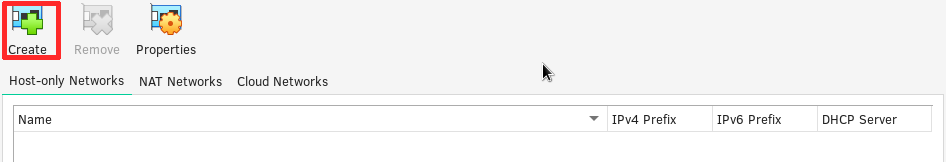
\includegraphics[width=0.8\textwidth]{graphics/setup/network-create.png}
  \caption{Erstellen des virtuellen Netzwerkadapters}\label{fig:network-host-manager}
\end{figure}

Danach kann man über \inlinecodee{Properties} die in Abb. \ref{fig:network-hm-properties} zu sehenden Einstellungen eintragen.

\begin{figure}[H]
  \centering
  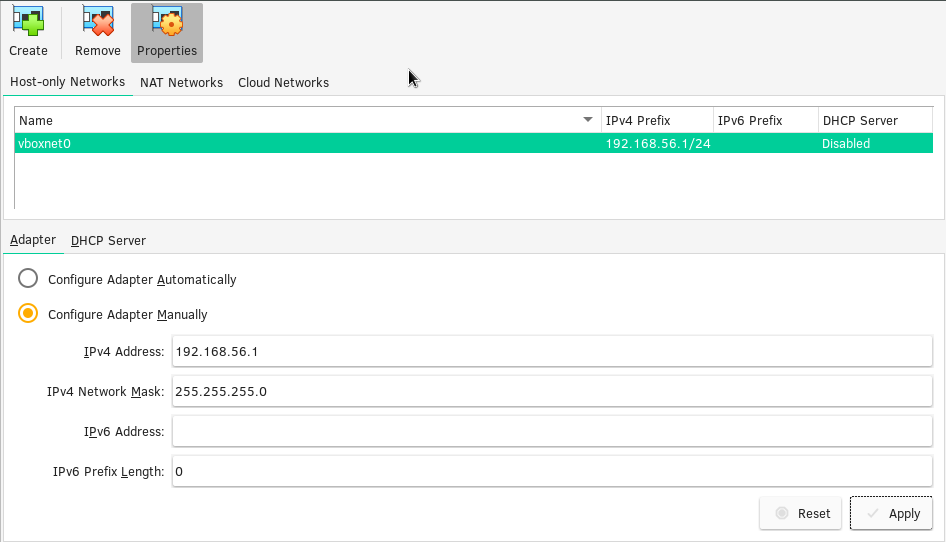
\includegraphics[width=0.8\textwidth]{graphics/setup/network-adapter.png}
  \caption{Einstellungen des Netzwerkadapters}\label{fig:network-hm-properties}
\end{figure}

Um die drei Hosts mit dem neuen virtuellen Adapter zu verbinden, wählt man die jeweilige Maschine aus, öffnet \inlinecodee{Settings} und wechselt zum \inlinecodee{Network}-Tab. Danach wählt man \inlinecodee{Adapter 2}, aktiviert ihn, setzt \inlinecodee{Attached to:} auf \inlinecodee{Host-only Adapter} und wählt den vorher erstellten Adapter aus (Abb. \ref{network-host-setup1}, \ref{network-host-setup2})

\begin{figure}[H]
  \begin{minipage}[t]{0.45\textwidth}
    \centering
    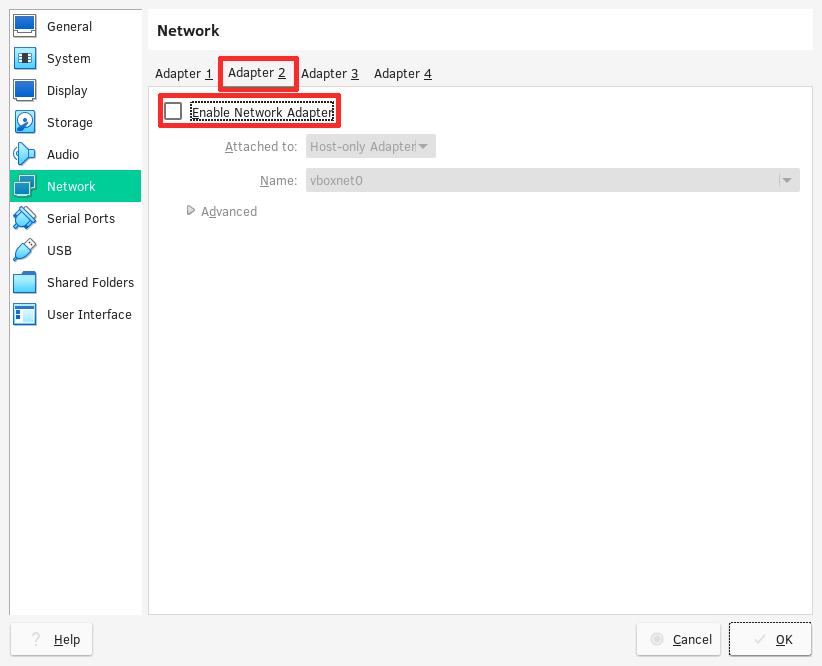
\includegraphics[width=\textwidth]{graphics/setup/network-host-setup1.png}
    \caption{Aktivieren von Adapter 2.}\label{network-host-setup1}
  \end{minipage}\hfill
  \begin{minipage}[t]{0.45\textwidth}
    \centering
    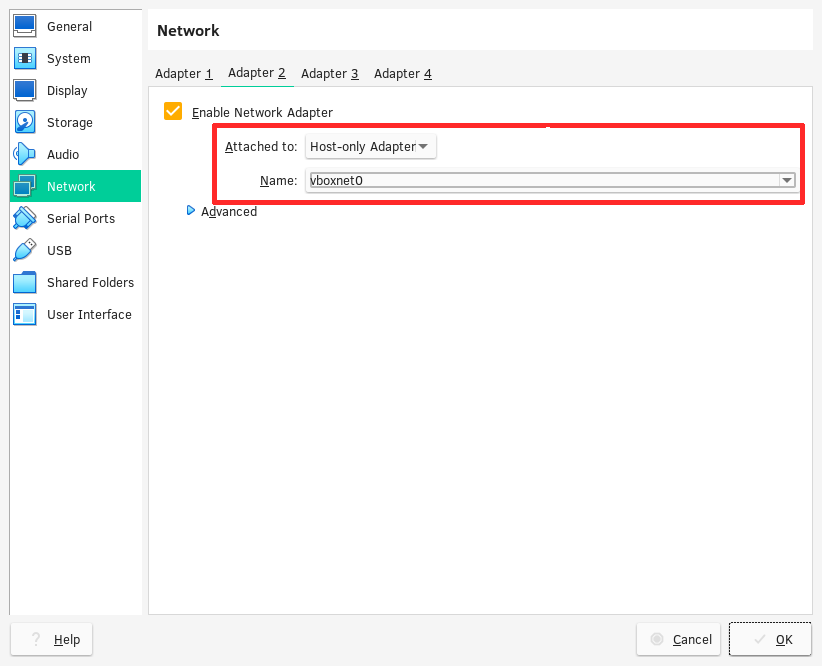
\includegraphics[width=\textwidth]{graphics/setup/network-host-setup2.png}
    \caption{Auswählen des Adapters.}\label{network-host-setup2}
   \end{minipage}
\end{figure}

Damit snort den Netzwerktraffic anderer Hosts sniffen kann, muss zuletzt für die NIDS-Maschine der Promiscuous-Modus aktiviert werden (Abb. \ref{fig:promisc}).

\begin{figure}[H]
  \centering
  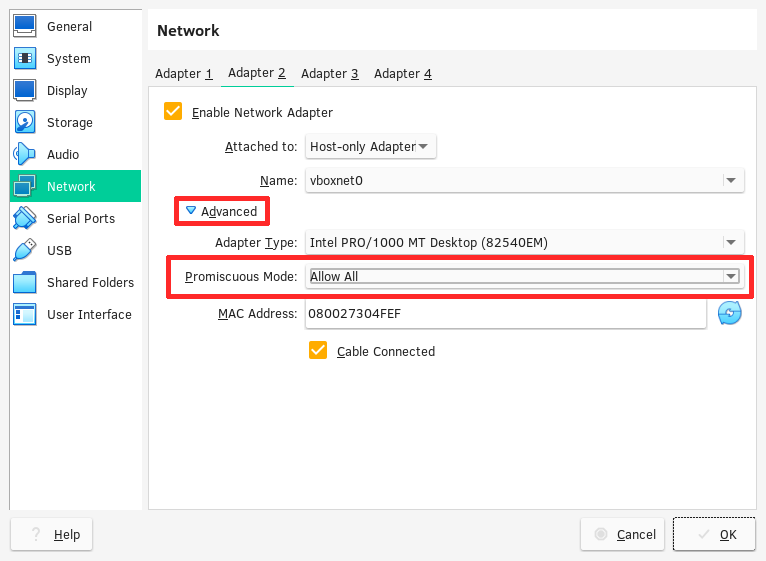
\includegraphics[width=0.5\textwidth]{graphics/setup/promisc.png}
  \caption{Promiscuous Mode für den NIDS-Host.}\label{fig:promisc}
\end{figure}


\subsection{IP-Adressen-Vergabe}\label{sec:ip-dist}
Jeder Host erhält eine statische IP-Adresse aus Reproduzierbarkeitsgründen. Diese können Tabelle \ref{tab:host-config} entnommen werden. Hierzu muss zuerst die Adapterbezeichnung auf der jeweiligen Maschine herausgefunden werden. Dies gelingt mit dem Befehl \inlinecodee{ip addr show} (Abb. \ref{fig:ip-addr-show})

\begin{figure}[H]
  \centering
  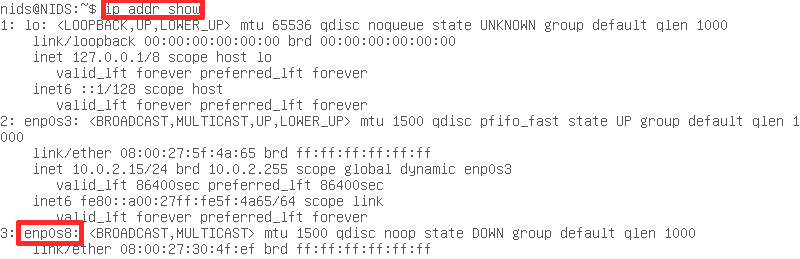
\includegraphics[width=0.8\textwidth]{graphics/setup/static-ip-1.png}
  \caption{VM-Netzwerkinterfaces.}\label{fig:ip-addr-show}
\end{figure}

Danach muss die Datei \inlinecodee{/etc/network/interfaces} entsprechend Abb. \ref{fig:static-ip-1} bearbeitet werden und der \inlinecodee{networking} Service neugestartet werden.

\begin{figure}[H]
  \centering
  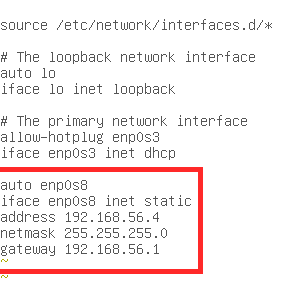
\includegraphics[width=0.25\textwidth]{graphics/setup/static-ip-2.png}
  \caption{\inlinecodee{/etc/network/interfaces}.}\label{fig:static-ip-1}
\end{figure}


\begin{minted}{bash}
    $ sudo systemctl restart networking.service
\end{minted}

Wurde dies für alle VMs durchgeführt, kann ein einfacher Verbindungstest über den \inlinecodee{ping}-Befehl ausgeführt werden.

\begin{table}
  \centering
\begin{tabular}{|l|l|l|l|l|l|}
\hline
ID  & OS & Hostname & user & password & IP \\ \hline
VM1 & Kali Linux & Attacker & attacker & 0000 &  192.168.56.2 \\ \hline
VM2 & Debian & Victim & victim & 0000 & 192.168.56.3 \\ \hline
VM3 & Debian & NIDS & nids & 0000 &192.168.56.4 \\
\hline
\end{tabular}
\caption{Zusammenfassung der Host-Konfigurationen}\label{tab:host-config}
\end{table}

